\section{Discussion}
\label{sec:Discussion}
% Our claims
The asymptotic dynamics of our model are affected by the strength of intraspecific competition compared to interspecific competition. Interestingly, we find that competition close to neutrality significantly increases the chances of chaotic behaviour. This suggests that in a system with predation, neutrality-on-average at the competition level may increase the probability of complex dynamics if the species are not equally prone to predation. We also found a clear correlation between non-stable dynamics and a higher prey biodiversity, being chaotic dynamics more efficient than cyclic at harboring a higher biodiversity. This allows us to conclude that chaos improves the chances for a higher number of coexisting species in our model. These observations, when put together, suggest that the hypothesis of non-equilibrium \citep{Huisman1999} and Hubbell's hypothesis of neutrality are not completely independent (see figure \ref{fig:GapInKnowledge}). 

%% Limitations
In the spirit of mathematical modelling, we chose the simplest realization required for the effects to be observed. We explored the variation away from neutrality only along the stabilizing/destabilizing axis. We didn't use Allee effect, nor noise, nor species-specific carrying capacities, and the functional form of each term has been chosen to account for satiation and saturation in the simplest possible ways. This opens the door to perform similar analyses in the future using more sophisticated models.

Both the competition and predation parameter sets were drawn from probability distributions. The interactions in our system can be interpreted as a weighted network with a high connectivity. In nature, trophic networks tend to show modular structure with various clusters \citep{Thebault2010}. Our simplified model could be interpreted as representing one of those densely connected modules. It is known that the asymptotic behaviour of this kind of systems can be very sensitive to the parameters choice. In particular, introducing correlations between parameters can greatly modify the probabilities of chaotic attractors to be reached (see for instance \citet{Huisman2001}, in response to the letter \citet{Schippers2001}). In the present paper we didn't introduce any correlation, i.e., all our random parameters were drawn independently from the others. Studying the effect of different physiological scenarios (in the sense of \citet{Huisman2001}, that is, constrains between the parameters) on the probabilities of chaos could be a continuation to this paper.

% Chaos detection
Due to the large number of simulations made, we had to rely on automatic methods for detecting chaos. Automatic detection of chaos by numerical methods has fundamental limitations, especially for high dimensional systems like ours. Most of them can be boiled down to the fact that, in general, numerical methods cannot distinguish robustly between long, complicated transients and genuine chaos. Our motivation to chose the Gottwald - Melbourne test \citep{Gottwald2009} was threefold: it escalates easily to systems of higher dimensions, its computation is fast and its conclusions fit better than any other method we tried when compared to the visual inspection of the time series. We think that our approach to chaos detection, despite being open to improvement, suffices to detect the overall patterns (see section \ref{subsec:ChaosDetection} in the Online Appendix for a more detailed discussion).

% Concluding remark
Our results suggest a fundamentally new way in which neutrality-on-average may promote biodiversity. In addition to weakening the forces of competitive exclusion \citep{Scheffer2018}, our analyses reveal that near neutrality may boost the chances for chaotic and cyclic dynamics. As chaos and cycles may facilitate super-saturated co-existence, our findings point to a potentially widespread mechanism of maintaining biodiversity.

\begin{figure}
	\begin{center}
		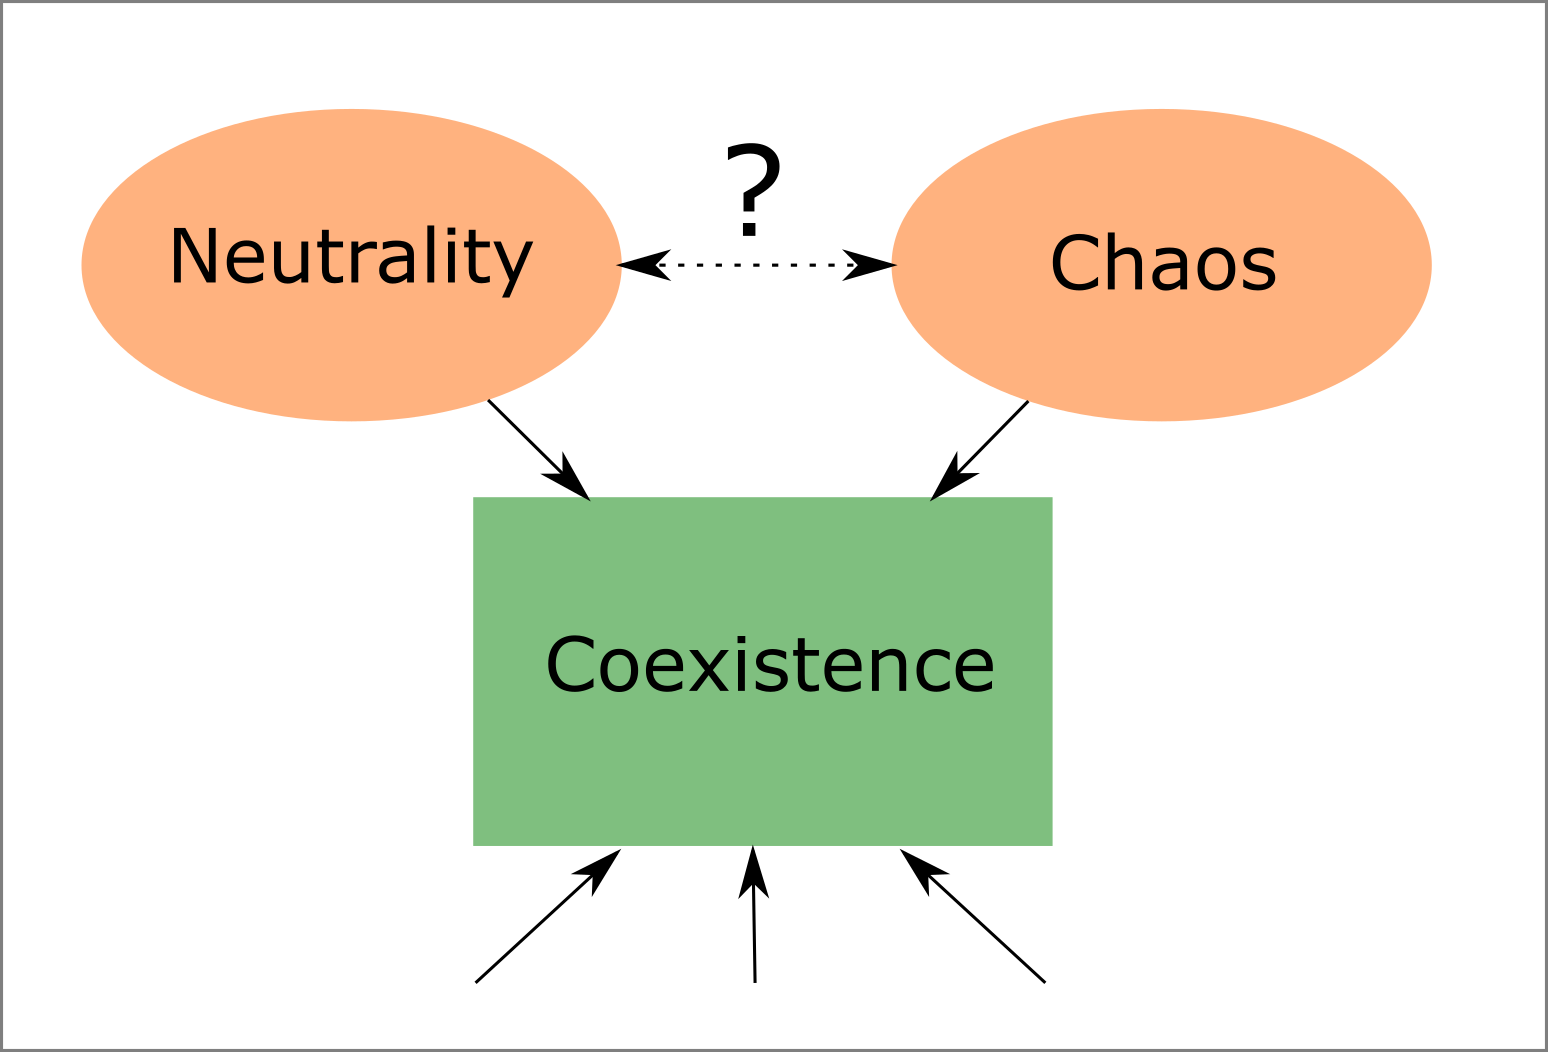
\includegraphics[width=0.5\columnwidth]{graphical_abstract.png}
	\end{center}
	\caption{In our model, neutrality and chaos are not independent explanations of coexistence.}
	\label{fig:GapInKnowledge}
\end{figure}
